\chapter{Feature Engineering and Exploratory Data Analysis}
This chapter discusses the process of feature engineering, which involves techniques such as feature scaling and feature transformation are described, which can help to normalize the range and distribution of features. Data visualization is also emphasized as a tool for gaining insights into the data, with examples given of how boxplots, distribution plots, and heat maps can be used to identify patterns and relationships in the data.

\section{Dataset Exploration}
Basic statistics of each features are shown below:

\begin{table}[H]
    \begin{center}
        \begin{tabular}{ |c|c|c|c|c|c|c| }
            \hline
            stats      & 
            fixed acidity&	volatile acidity	&citric acid&	residual sugar&	chlorides	&free sulfur dioxide  \\
            \hline
            mean & 8.311	& 0.5313	& 0.264 &	2.532 &	0.0869	& 15.615 \\
            \hline

            std & 1.747	&0.179&	0.196&	1.355	&0.0477&	10.250 \\
            \hline

            min & 4.600&	0.120000	&0.000&	0.900	&0.0120&	1.00 \\
            \hline

            25\% & 7.100	&0.39250 & 0.0900 &	1.900	&0.070&	7.000 \\
            \hline

            50\% & 7.900 &	0.5200&0.2500	&2.200&	0.0790&13.000	 \\
            \hline

            75\% & 9.100	&0.6400&0.4200&2.6000&0.090	&21.000	 \\
            \hline

            max & 15.900 &	1.580	&1.00&	15.50&	0.6110	&68.00 \\
            \hline
        \end{tabular}
    \end{center}
    \caption{Data Description 1}
    \label{table:Data Description 1}
\end{table}


\begin{table}[H]
    \begin{center}
        \begin{tabular}{ |c|c|c|c|c|c| }
            \hline
            stats      & 
            total sulfur dioxide	&density&	pH	&sulphates&	alcohol	  \\
            \hline
            mean & 45.914698	&0.996730&	3.311015	&0.657708	&10.442111 \\
            \hline

            std & 32.782130	&0.001925&	0.156664&	0.170399&	1.082196	\\
            \hline

            min & 6.000000	&0.990070	&2.740000&	0.330000	&8.400000	 \\
            \hline

            25\% & 21.000000	&0.995570&	3.205000	&0.550000&	9.500000	 \\
            \hline

            50\% & 37.000000	&0.996680&	3.310000	&0.620000&	10.200000		 \\
            \hline

            75\% & 61.000000&	0.997845&	3.400000&	0.730000&	11.100000		 \\
            \hline

            max & 289.000000 &	1.003690&	4.010000&	2.000000&	14.900000	 \\
            \hline
        \end{tabular}
    \end{center}
    \caption{Data Description 2}
    \label{table:Data Description 2}
\end{table}

The correlation between data is shown in following heat map.
\begin{figure}[H]
    \centering
    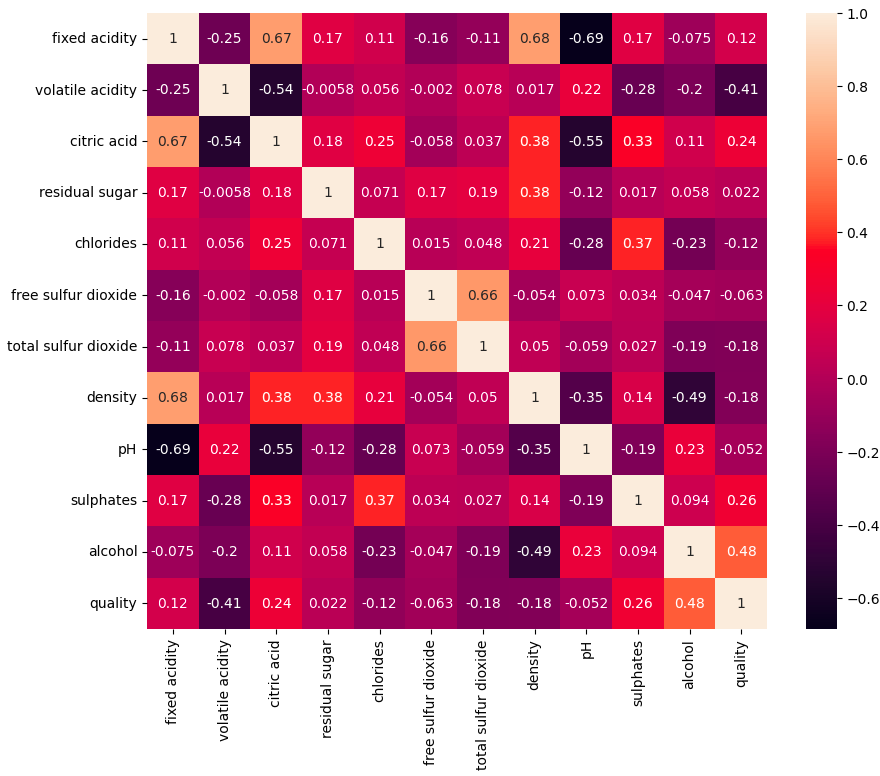
\includegraphics[scale = 0.5]{preprocessing/corr_heat_map.png}
    \caption{Correlation Heat Map}
    \label{fig:Correlation Heat Map}
\end{figure}

\begin{figure}[H]
    \centering
    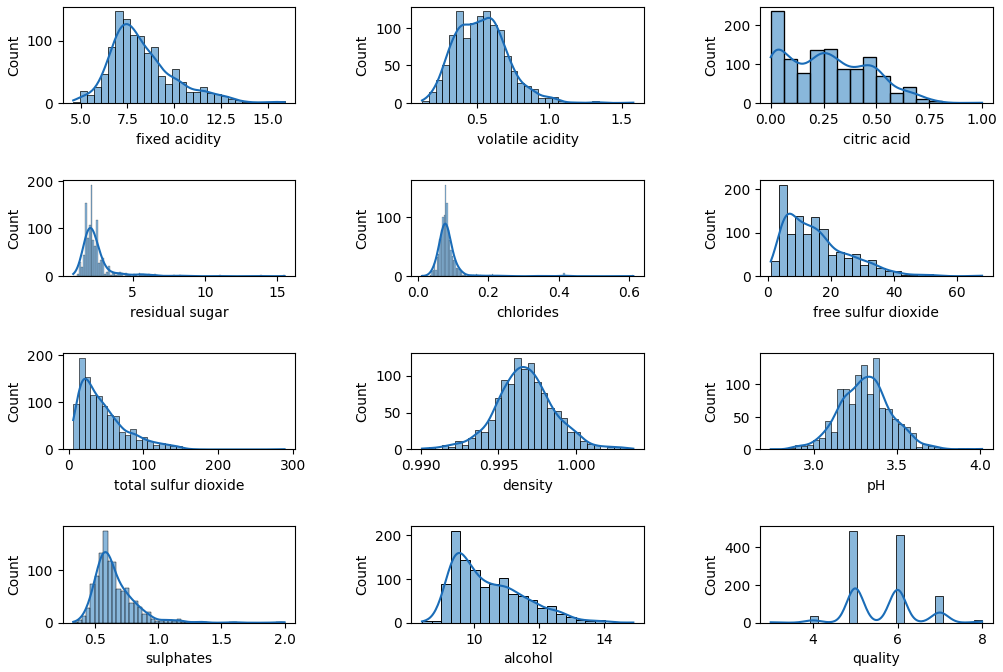
\includegraphics[scale = 0.4]{preprocessing/original_data_untransformed_distribution.png}
    \caption{Distribution Plot of the entire datasets}
    \label{fig:Distribution Plot of the entire datasets}
\end{figure}

\begin{figure}[H]
    \centering
    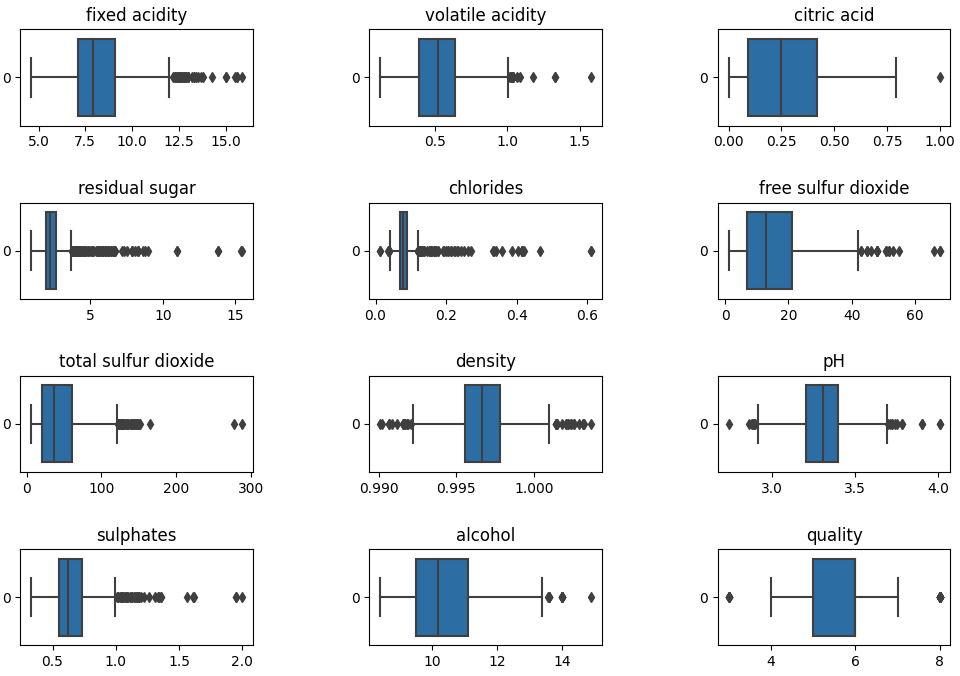
\includegraphics[scale = 0.4]{preprocessing/boxplot_whole_data.png}
    \caption{Box Plot of the entire datasets}
    \label{fig:Box Plot of the entire datasets}
\end{figure}

\section{Min Max Scaling}
Min max scaling was used as it scales all the data features in the range of 0 and 1 due to which it becomes easier to transform the data using log transformation and boxcox transformation. We can see how data have been normalized and outliers have been handled from following plots

\begin{figure}[H]
    \centering
    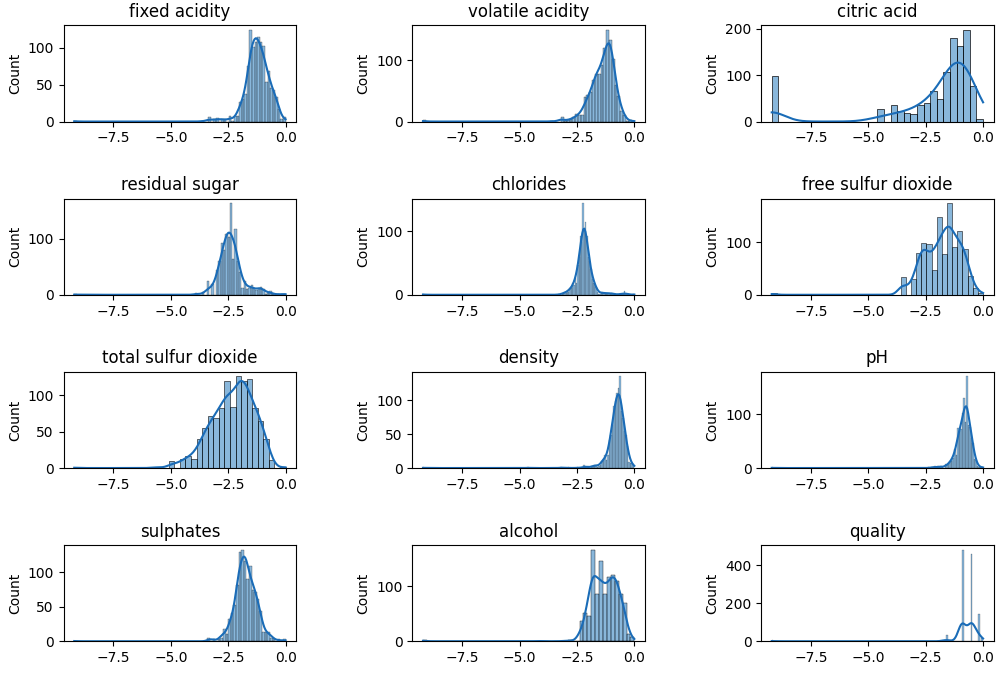
\includegraphics[scale = 0.35]{preprocessing/min_max_scaled/dist_log_transformed_data.png}
    \caption{Distribution Plot of log transformed data after minmax scaling}
    \label{fig:Distribution Plot of log transformed data after minmax scaling}
\end{figure}

\begin{figure}[H]
    \centering
    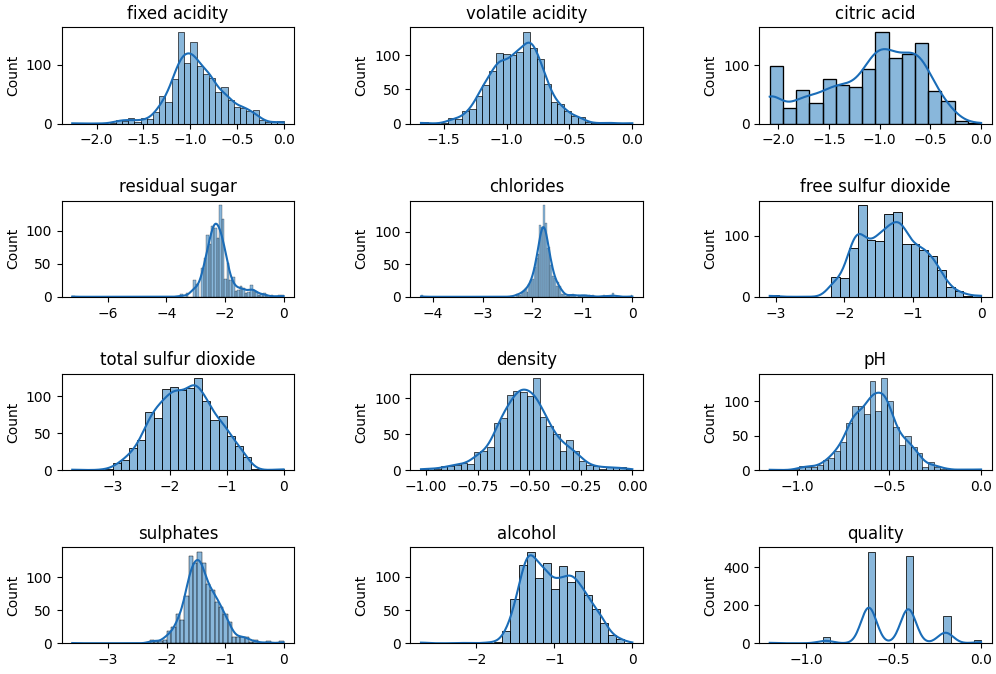
\includegraphics[scale = 0.35]{preprocessing/min_max_scaled/dist_boxcox_transformed.png}
    \caption{Distribution Plot of boxcox transformed data after minmax scaling}
    \label{fig:Distribution Plot of boxcox transformed data after minmax scaling}
\end{figure}

\begin{figure}[H]
    \centering
    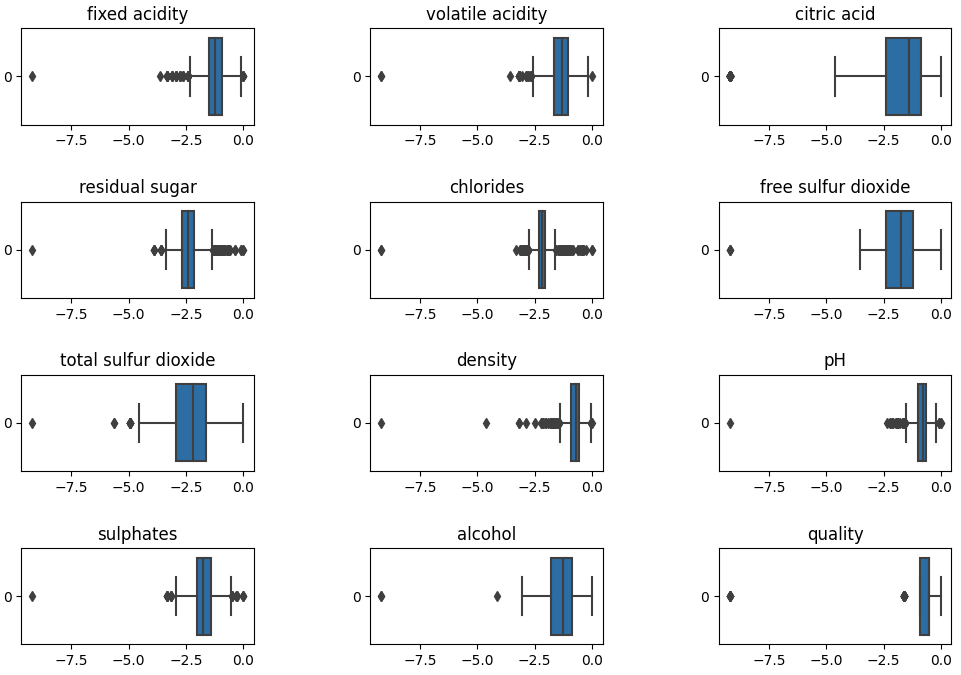
\includegraphics[scale = 0.4]{preprocessing/min_max_scaled/boxplot_log_transformed.png}
    \caption{Box Plot of log transformed data after minmax scaling}
    \label{fig:Box Plot of log transformed data after minmax scaling}
\end{figure}

\begin{figure}[H]
    \centering
    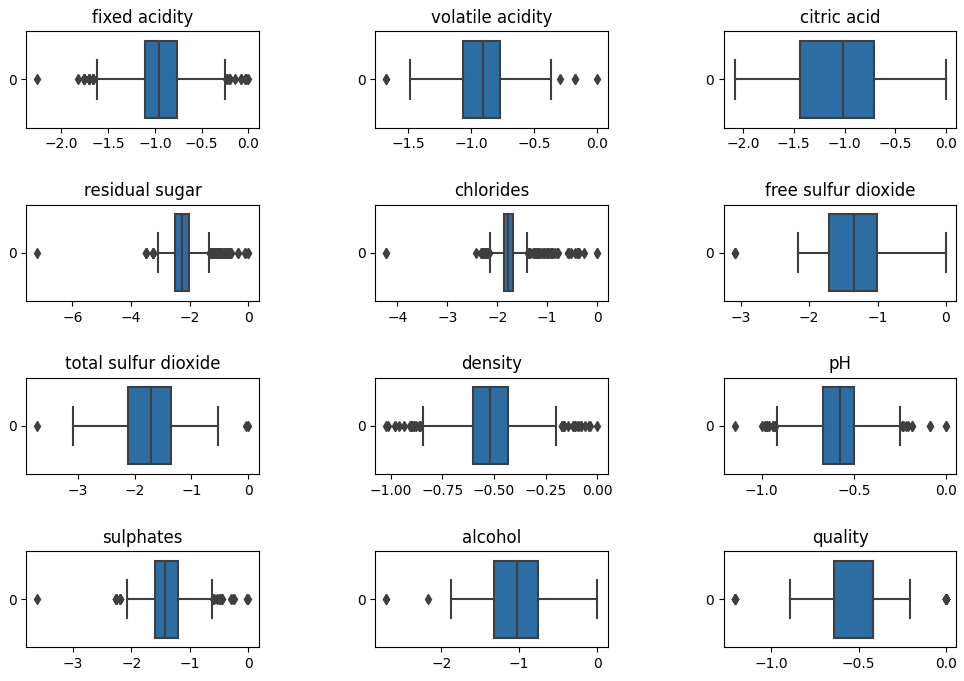
\includegraphics[scale = 0.4]{preprocessing/min_max_scaled/boxplot_boxcox.png}
    \caption{Box Plot of boxcox transformed data after minmax scaling}
    \label{fig:Box Plot of boxcox transformed data after minmax scaling}
\end{figure}


